\documentclass[11pt]{beamer}
\usepackage[utf8]{inputenc}
\usepackage{movie15}
%\usepackage[english]{babel}
\usepackage{graphicx}
\usetheme{Madrid}
\usepackage[T1]{fontenc}
\usepackage[ngerman]{babel}
%\usepackage{xcolor}
\makeatletter
\def\ScaleIfNeeded{%
\ifdim\Gin@nat@width>\linewidth
\linewidth
\else
\Gin@nat@width
\fi
}
\makeatother

\begin{document}
    \author{C. Bojko, D. Pape}
    \title{\textbf{Google - Suchalgorithmen \& Privacyprobleme}}
  %  {------------------------------------------------------}
    %\subtitle{}
    %\logo{}
    %\institute{}
    %\date{}
    %\subject{}
    %\setbeamercovered{transparent}
    %\setbeamertemplate{navigation symbols}{}
    \frame[plain]{\maketitle}
    
\begin {frame}
        \frametitle{\ Übersicht}

\begin{description}
%\vspace{0.3cm}
\item[•]Suchalgorithmus
\item[•]Privacyprobleme
\end{description}
\end{frame}

\begin{frame}{Suchalgorithmus}

    \begin{block}{Definition \dq How Google Search Works\dq - by Google}
    \dq Every time you search, there ae thousands, sometimes millions, of webpages with helpful information. How Google figures out which results to show starts long before you even type, and is guided by a commitment to you to provide the best information.\dq
    \end{block}
    
\end{frame}

\begin{frame}{Website \dq crawling\dq}
    \begin{block}{Crawling}
        Der Crawling-Prozess beginnt mit einer Liste von Webadressen aus früheren Crawls und Sitemaps. Er besucht Websites, benützt Links zu neuen Websites und \dq springt\dq\  sozusagen immer weiter. Weitere Programme werten den Inhalt aus und verarbeiten die Daten.
    \end{block}
    \begin{alertblock}{Sitemaps}
    Eine Datei in der Informationen über die Seiten, Videos und anderen Dateien und deren zusammenhang stehen. Sie helfen der Google-Suche wichtige Informationen von der Website leichter zu finden.
    \end{alertblock}
\end{frame}


\begin{frame}{Indexing}
    \begin{block}{Indexing}
        Die im Crawling-Prozess gesammelte Information wird in einem gigantischen Index gesammelt, der auf sehr viele Rechner verteilt ist. Die Informationen sollen widerspiegeln, was das Thema einer Seite ist.
    \end{block}
    
\end{frame}

\begin{frame}{Ranking}
    \begin{block}{Geschichte - PageRank}
        PageRank war der ursprüngliche Suchalgorithmus von Google in den 90ern. Die Neuheit von PageRank war, dass Seiten nach der Anzahl \textit{Backlinks} gereiht wurden.
    \end{block}
    
    \begin{block}{Backlinks}
        Eine Seite $S$ hat $n$ Backlinks, wenn es $n$ Links zu $S$ gibt.
    \end{block}
    
    In PageRank wurde jedem Backlink auch ein Gewicht zugewiesen - wenn die Seite, von der der Backlink stammt, selbst \dq wichtig\dq ist, dann zählt ein solcher Backlink mehr als ein Backlink von einer unwichtigen Seite.
\end{frame}

\begin{frame}{Ranking - Probleme}

    \begin{block}{Missbrauchspotenzial}
        Da Google akademische Ursprünge hat, war der PageRank Algorithmus öffentlich, und somit war es trivial, mit sog. Linkfarmen für den Algorithmus zu optimieren.
    \end{block}
    
    \begin{block}{Teilprobleme des Rankings}
        Das Ziel ist, die \textit{Relevanz} der Suchergebnisse für den Nutzer zu maximieren.
        \begin{itemize}
            \item Tippfehler
            \item Unterstützung von Natural Language Queries
            \item Mehrdeutige Begriffe
            \begin{itemize}
                \item \dq how to \textbf{change} a light bulb\dq
                \item \dq does post office \textbf{change} foreign currency\dq
                \item \dq how to \textbf{change} laptop brightness\dq
            \end{itemize}
        \end{itemize}
    \end{block}
\end{frame}

\begin{frame}{Ranking - Probleme}
    \begin{block}{Teilprobleme des Rankings}
        \begin{itemize}
            \item Wird spezifische/aktuelle Information gesucht?
            \begin{itemize}
                \item Eine Suche nach \dq bundesliga\dq oder \dq apple aktie\dq erfordert aktuelle Information
                \item \dq burgerista öffnungszeiten\dq fordert einen spezifischen Datenpunkt
                \item Ob aktuelle Information gesucht wird, wird u.A. daran festgestellt, ob die Such-Keywords \textit{trending} sind.
            \end{itemize}
        \end{itemize}
    \end{block}
    
    Mit der Zeit wurden viele Updates zum Algorithmus eingeführt, die dieses Probleme beheben sollten.
\end{frame}


\begin{frame}{Updates zum Suchalgorithmus}
    \begin{block}{Panda (2011)}
        Bewertung der \textit{Qualität} von Seiten:
        \begin{itemize}
            \item Ist die SEO sauber? (Metadaten, ...)
            \item Formulierung der Texte
            \item Qualität der Grafiken
            \item Sind die Unterseiten einander ähnlich?
            \item Wie lange bleiben die Besucher im Allgemeinen?
        \end{itemize}
    \end{block}
    
    \begin{block}{Penguin (2012)}
        Abwertung von Seiten, die \dq Black Hat \dq SEO einsetzen:
        \begin{itemize}
            \item Texte künstlich mit übermäßig vielen Keywords anreichern
            \item für die Nutzer unsichtbare Texte in die Seite einzubauen, um mehr Keywords unterzubringen (z.B. mit white-on-white text)
        \end{itemize}
    \end{block}
\end{frame}

\begin{frame}{Updates zum Suchalgorithmus}
    \begin{block}{Hummingbird (2013)}
        Erlaubte Suchen nicht nur per Keyword, sondern per Semantik: z.B. könnte man statt \dq wm 2014 gewinner \dq nach \dq wer hat die wm 2014 gewonnen \dq suchen und auf sinnvolle Ergebnisse hoffen.
    \end{block}
    
    
    \begin{block}{RankBrain (2015)}
        ML/AI für Ranking:
        \begin{itemize}
            \item Ziel: Bessere Bearbeitung von zuvor unbekannten Suchanfragen
            \begin{itemize}
                \item 15\% aller Anfragen wurden vorher noch nie gesehen!
            \end{itemize}
            \item AI soll die Semantik der Anfrage analysieren
            \item So können ähnliche zuvor beantwortete Anfragen zur Hilfe gezogen werden
        \end{itemize}
    \end{block}
\end{frame}

\begin{frame}{Ranking}
    Heutzutage ist der Suchalgorithmus also klüger geworden und versteht auch den Inhalt der Seiten. Damit ist Black Hat SEO weniger effektiv. Weiters ist die genaue Funktionsweise nicht mehr öffentlich. Bekannt ist aber, dass u.a. folgende Variablen berücksichtigt werden:
    
    
    \begin{block}{Berücksichtigte Variablen}
        \begin{itemize}
            \item Standort
            \begin{itemize}
                \item Eine Suche nach \dq bicycle repair shop\dq in Paris sollte ganz andere Ergebnisse liefern als eine in Tokio. 
                \item Allerdings sollte dies für eine Suche nach \dq last nobel prize winner\dq nicht der Fall sein.
            \end{itemize}
            \item Datum und Zeit
            \begin{itemize}
                \item Eine Suche nach \dq wm sieger\dq  sollte den Sieger der \textit{letzten} WM finden.
            \end{itemize}
            \item Sprache
        \end{itemize}
    \end{block}
\end{frame}

\begin{frame}{Ranking}    
    \begin{block}{Berücksichtigte Variablen}
        \begin{itemize}
            \item Vorherige Suchanfragen
            \begin{itemize}
                \item Liefern Kontext
                \item Wiederholte Anfragen bedeuten, dass vorherige Suchen nicht das richtige Ergebnis geliefert haben
            \end{itemize}
            \item Gerät des Nutzers
            \begin{itemize}
                \item Hauptsächlich geht es um Desktop, Tablet oder Mobile
                \item Beispielsweise werden mobile-friendly Seiten bevorzugt, wenn der Nutzer auf einem Mobilgerät ist.
            \end{itemize}
        \end{itemize}
    \end{block}
\end{frame}

\begin{frame}{Privacyprobleme}
    \begin{block}{Was sind Privacyprobleme}
            Privacyprobleme konzentrieren sich auch die Offenlegung der genetischen Informationen eines Users an Dritte.
    \end{block} 
    \begin{block}{Google's privacy policy (March 1, 2012)}
            Seit 2012 kann Google Daten über eine Vielzahl von Diensten weitergeben. Dazu gehören Websites Dritter, die Adsense oder Google Analytics verwenden. 
    \end{block}
    \begin{alertblock}{Eric Schmidt - Google CEO 2009}

    \dq If you have something that you don't want anyone to know, maybe you shouldn't be doing it in the first place.\dq‚
    \end{alertblock}
\end{frame}

\begin{frame}{Cookies}
    \begin{block}{Was sind Cookies}
            Ein Cookie ist eine Textinormation, die im Browser eines Endgerätes zu einer Besuchten Website gespeichert werden kann. Dies kann entweder vom Webserver an der Browser oder direkt im Browser mit einem Javascript erstellt werden. Bei wiederholtem aufrufen einer Website kann der Server diese Datei auslesen.
    \end{block} 
    \begin{block}{Welche Daten werden gespeichert?}
            Cookies können eine Vielzahl von Informationen beinhalten. Unter anderem können persönliche Daten wie Name, Adresse, Email oder Telefonnummer gespeichert werden. Jedoch hat eine Website nur zu den Cookies zugriff die Sie selbst bereitstellen.
    \end{block}
\end{frame}

\begin{frame}{Cookies}
    \begin{block}{Cookies bei Google}
        \begin{itemize} 
        \item Google platziert eins oder mehrere Cookies auf dein Rechner eines Users
        \item Dadurch kann sein Suchverlauf und der Besuch auf Websites gespeichert werden.
        \item Wenn ein Google Konto verknüpft ist werden alle besuchten Websites und alle Suchen dazu gespeichert.
        \item Seit 2016 informieren Googles Datenschutzrichtlinien nicht, ob und wann solche Aufzeichnungen gelöscht werden.
        \item Diese Informationen werden, auf Anfrage, Strafverfolgungsbehörden weitergeleitet.
        \end{itemize}
    \end{block}



\end{frame}

\begin{frame}{Tracking}
    \begin{block}{Wie verwendet Google Tracking?}
        Tracking kann durch verschiedene Tools von Google genutzt werden. Unter anderem durch Analytics, Play Services, reCAPTCHA, Google Fonts und APIs. Durch diese Tools kann Google die Route, die ein User nützt ermitteln. Durch die große Anzahl von Diensten und Websiten die zu Google gehören, ist es sehr schwer nachzuvollziehen wo die Informationen hingehen.
    \end{block}
    \begin{block}{Ein Trick von Google}
        Als Beispiel gibt es das ReCAPTCHA von Google. Dieses Tool verwendet als Domaine "www.google.com" was bedeutet sie können Cookies die von Google stammen benützen und erweitern, da sie die dadurch die Beschränkung, dass man Drittanbieter Cookies verändert, umgehen.
    \end{block}
\end{frame}

\begin{frame}{Google Mail}
    \begin{block}{Wie wird Google Mail wirklich verwendet}
    \begin{itemize}
        \item Google Mail wird rein für Marketing Zwecke benützt.
        \item Mail's werden zwar nicht von Menschen gelesen, jedoch werden sie von Computern analysiert.
        \item Dadurch kann ein User genauestens analysiert werden, da in den Mails meist private Gespräche vorhanden sind.
        \begin{itemize}
            \item EMails von Bestellungen (Amazon etc)
            \item Private Mails mit Freunden/Bekannten
        \end{itemize}
    \end{itemize}
    \end{block}
    \begin{alertblock}{Zitat Eric Schmidt Google CEO 2010}
    “We know where you are.  We know where you’ve been.
    We can more or less know what you’re thinking about.”
    \end{alertblock}
\end{frame}

\begin{frame}{Google Mail}
    \begin{block}{Third-Party Apps}
    2014 hat Google third-party Entwicklern Zugang zur GMail API gegeben. Dadurch     können sie Software erstellen, die innerhalb der Plattform verwendet werden     kann.
    \begin{itemize}
        \item Meist sind solche Softwares Produktivitäts-Tools. 
            \begin{itemize}
                \item Aufgabenmanager
                \item Apps zum Signieren von Dokumenten
            \end{itemize}
        \item Das Problem besteht darin, dass solche Apps beim installieren auch die Erlaubnis zum Lesen von Emails bekommen.
        \end{itemize}
    \end{block}
    \begin{alertblock}{Third-Party Entwickler}
    Nach einem Beitrag im Wall Street Journal im Jahr 2018 gab es einen Vorfall, wo ein Angestellter solcher Drittanbieter 8000 Emails durchgelesen haben um ihre Algorithmen zu verbessern.
    \end{alertblock}
\end{frame}

\begin{frame}{Google Chrome}
    \begin{block}{Google's Suchleiste}
    \begin{itemize}
        \item Chrome verfügt über eine kombinierte Such-/Adresszeile die auch Omnibar genannt wird.
        \item Google überträgt dabei in Echtzeit um die Sucheingabe zu vervollständigen.
        \item Der Gründer von Fluid New Media, Ahad Bokhari, fand durch das Testen des Browsers im Debug-Proxy Mode heraus, dass bei fast jedem Tastenschlag mit dem Server kommuniziert wird.
        \item Diese Daten kombiniert mit Cookies/Emails und Verlauf können ein sehr detailliertes Bild eines Users erstellen.
    \end{itemize}
    \end{block}
    
\end{frame}
\begin{frame}{Android}
    Android ist das mit rund 72\% am meisten genützte Smartphone OS. Es gibt rund 2,5 Milliarden aktive Android Geräte. \newline 
    Beispiel:
    \begin{itemize}
        \item The Associated Press hat herausgefunden, dass auch wenn man Standortinformationen deaktiviert, der Standort im Google Konto hinterlegt wird. Wenn auch etwas ungenauer.
        \item Eine App kann den Bildschirmstatus des Smartphones ohne jegliche Berechtigung überwachen.
        \item Eine App kann Ihre WiFi-/Mobilfunk-Datennutzung ohne jegliche Berechtigungen überwachen.
        \item Eine App kann eine Liste aller anderen auf Ihrem Telefon installierten Apps ohne jegliche Berechtigungen erhalten.
        \item Apps können ohne explizite Berechtigung abfragen in welchem Winkel und in welche Richtung das Telefon gehalten wird und ob es sich bewegt.
    \end{itemize}
\end{frame}

\begin{frame}{Statistiken}
    \begin{figure}
        \centering
        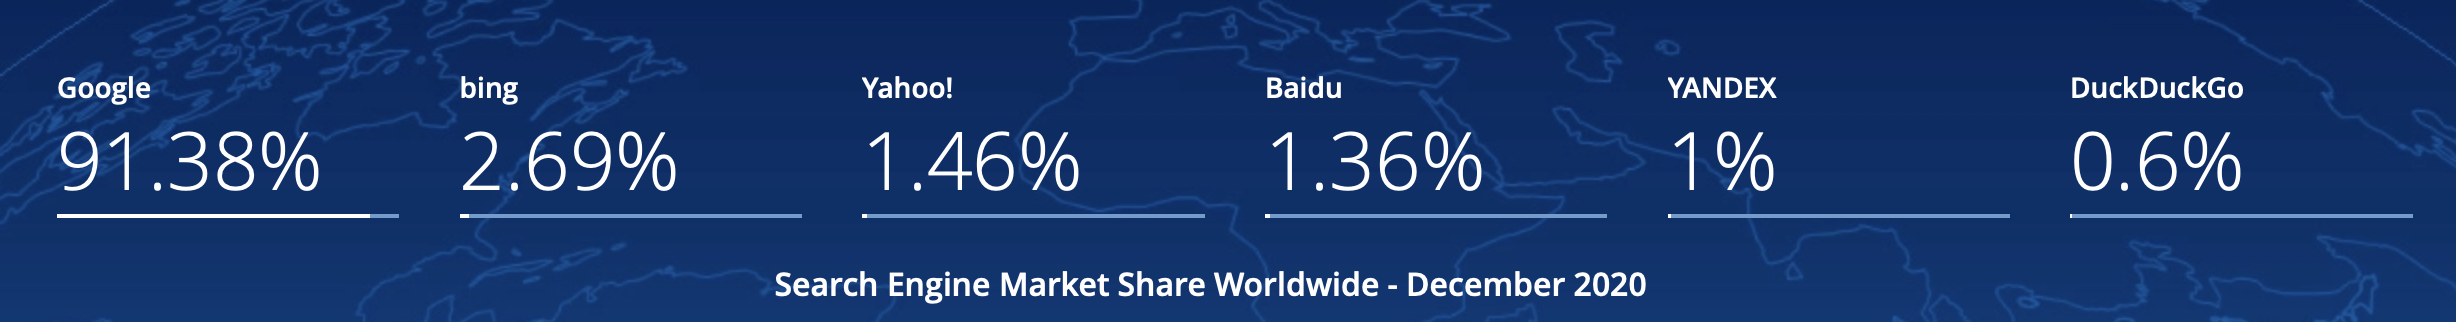
\includegraphics[width=\textwidth]{googlesearchmarketshare.png}
        \caption{\tiny https://gs.statcounter.com/search-engine-market-share}
    \end{figure}
    \begin{figure}
        \centering
        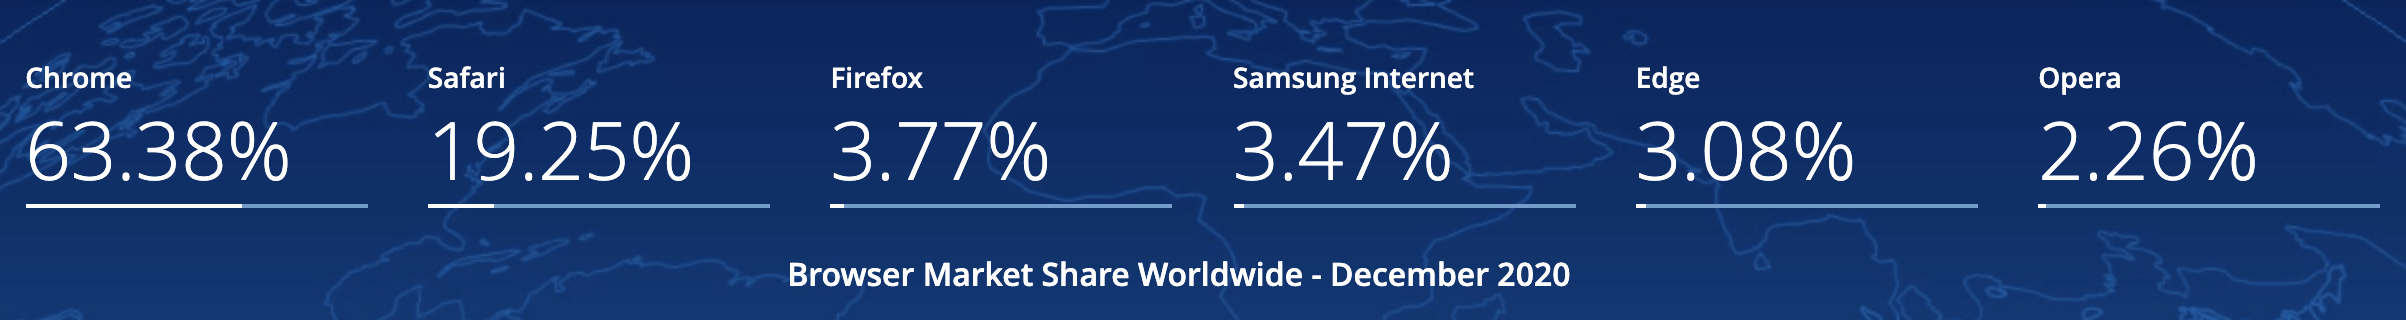
\includegraphics[width=\textwidth]{browsermarketshare.png}
        \caption{\tiny https://gs.statcounter.com/browser-market-share}
    \end{figure}

\end{frame}

\begin{frame}{Statistiken}
    \begin{figure}
        \centering
        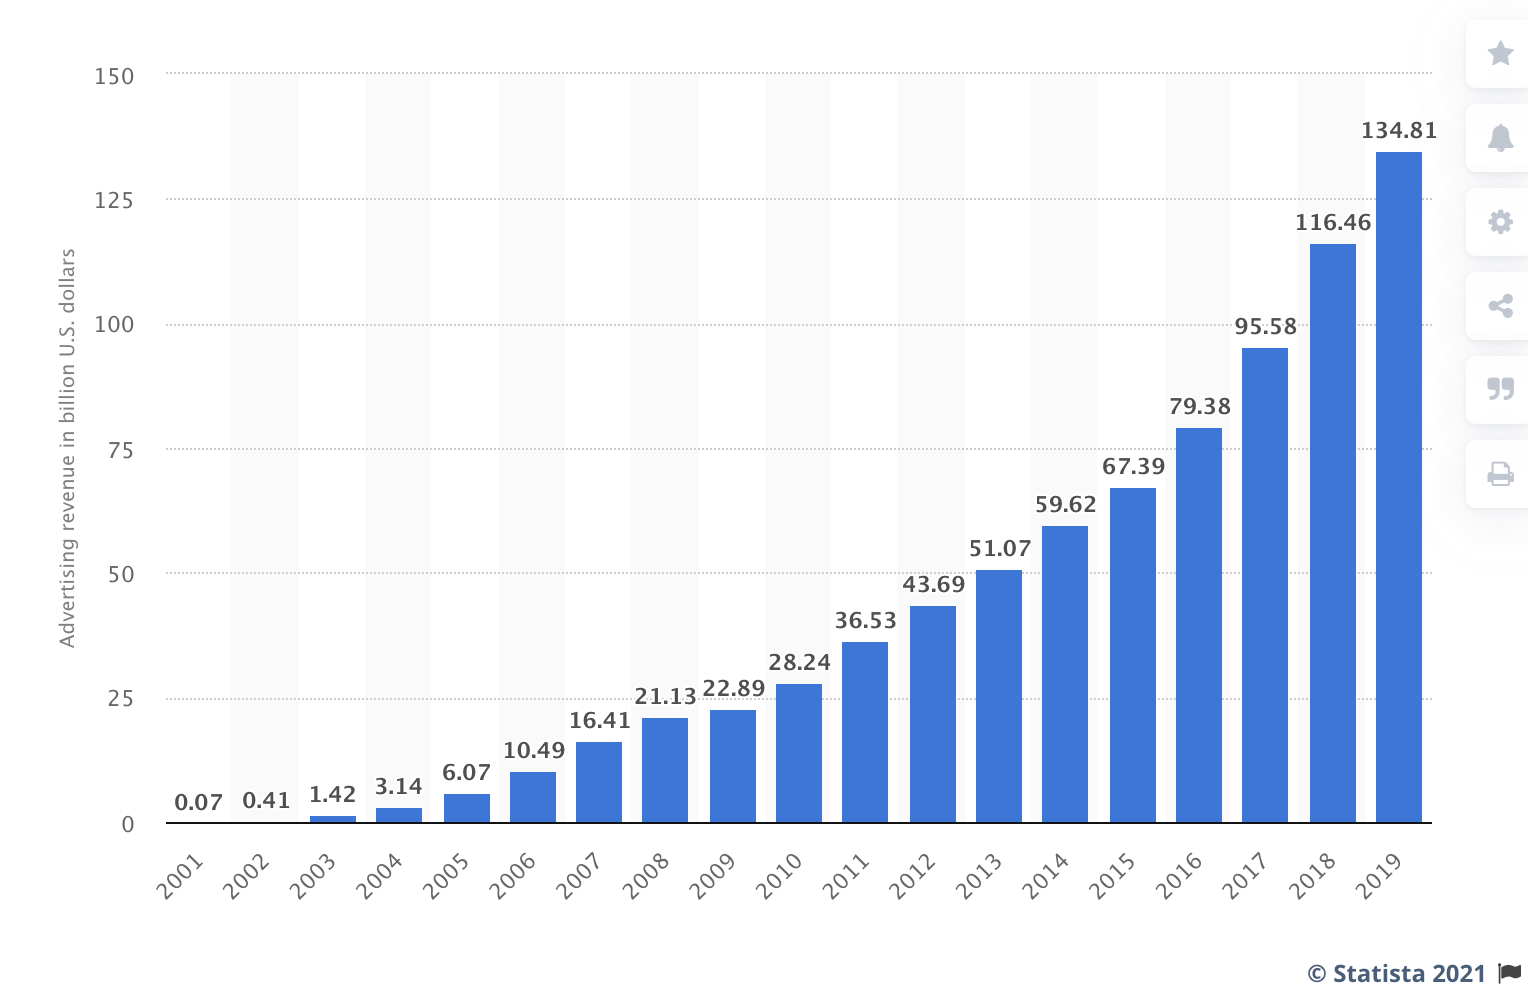
\includegraphics[scale=0.3]{googleadmoney.png}
        \caption{\tiny https://www.statista.com/statistics/266249/advertising-revenue-of-google/}
    \end{figure}
\end{frame}

\begin{frame}{Statistiken}
        \begin{figure}
        \centering
        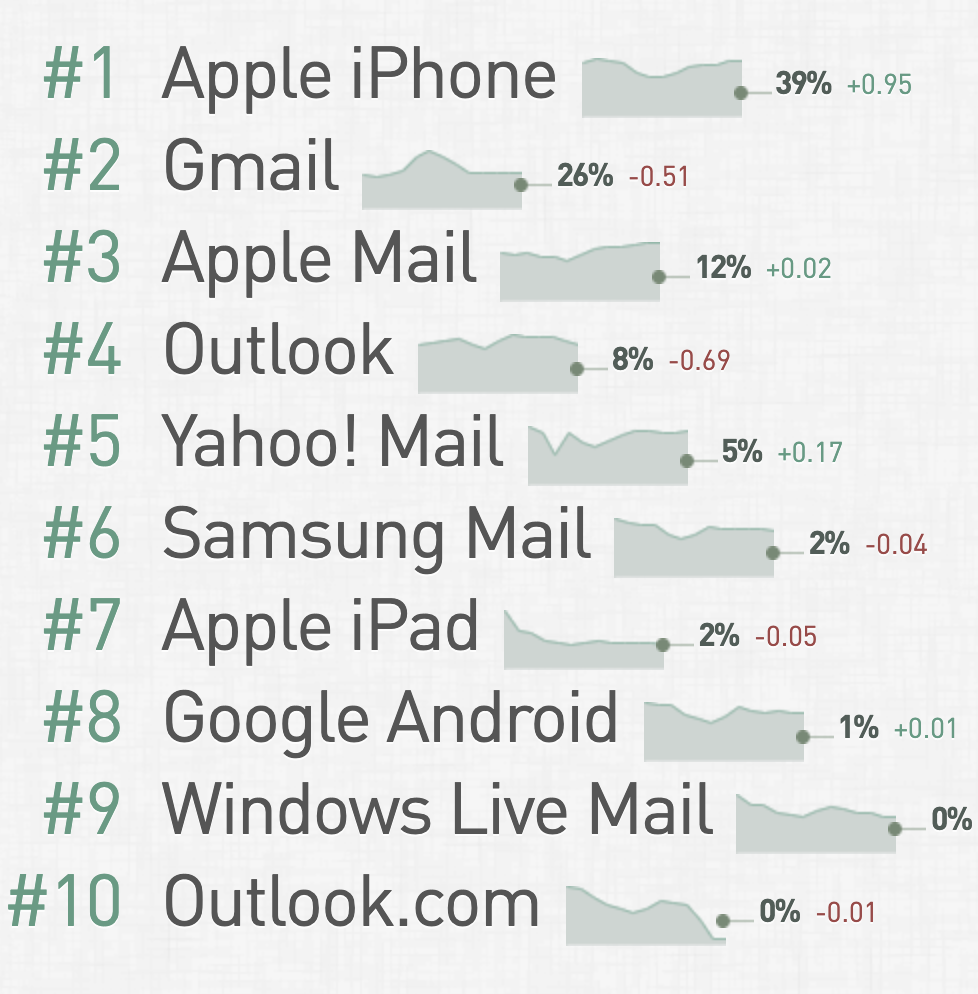
\includegraphics[scale=0.2]{gmailmarketshare.png}
        \caption{\tiny https://emailclientmarketshare.com/}
    \end{figure}

    \begin{figure}
        \centering
        \includegraphics[width=\textwidth]{phonemarketshare.png}
        \caption{\tiny https://gs.statcounter.com/os-market-share/mobile/worldwide}
    \end{figure}
\end{frame}



\begin{frame}{Referenzen}
    \begin{itemize}
    \tiny
        \item https://developers.google.com/search/docs/basics/how-search-works
        \item https://www.heise-regioconcept.de/google/wie-funktioniert-der-algorithmus-von-google
        \item https://www.google.com/search/howsearchworks/algorithms/
        \item https://protonmail.com/blog/google-privacy-problem/
        \item https://en.wikipedia.org/wiki/Privacy\_concerns\_regarding\_Google
        \item https://www.wsj.com/articles/techs-dirty-secret-the-app-developers-sifting-through-your-gmail-1530544442
        \item https://smallbusiness.chron.com/google-chrome-privacy-problems-28257.html
        \item https://www.theverge.com/2019/5/7/18528297/google-io-2019-android-devices-play-store-total-number-statistic-keynote
        \item https://gs.statcounter.com/os-market-share/mobile/worldwide
        \item https://gs.statcounter.com/browser-market-share
        \item https://emailclientmarketshare.com/
        \item https://github.com/databurn-in/Android-Privacy-Issues
    \end{itemize}
\end{frame}

\end{document}r
